\documentclass{standalone}
\usepackage{tikz}
\usepackage{xcolor}

\begin{document}
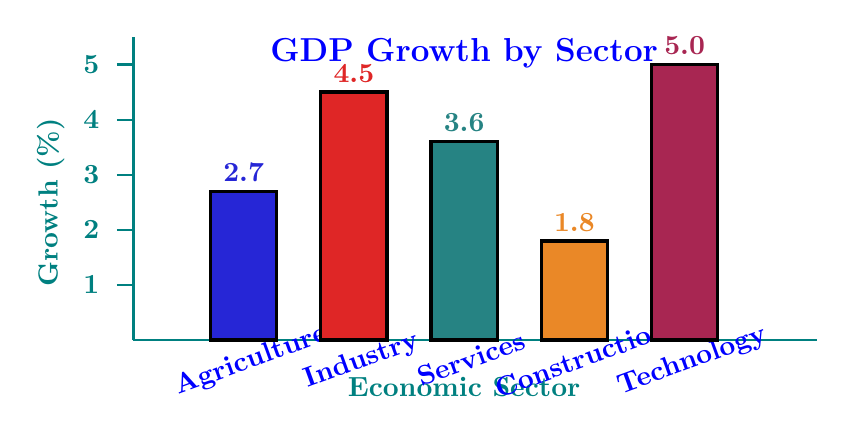
\begin{tikzpicture}[x=1.4cm, y=0.7cm]
% Define colors
\definecolor{agriculture}{RGB}{38,38,214}
\definecolor{industry}{RGB}{223,38,38}
\definecolor{services}{RGB}{38,131,131}
\definecolor{construction}{RGB}{234,136,39}
\definecolor{technology}{RGB}{168,38,82}
\definecolor{axiscolor}{RGB}{0,128,128}

% Title
\node[font=\bfseries\large, blue] at (3, 5.2) {GDP Growth by Sector};

% Y-axis
\draw[axiscolor, thick] (0,0) -- (0,5.5);
% Y-axis label
\node[axiscolor, rotate=90, font=\bfseries] at (-0.75, 2.5) {Growth (\%)};
% Y-axis ticks and labels
\foreach \y in {1,...,5} {
    \draw[axiscolor, thick] (-0.15,\y) -- (0,\y);
    \node[axiscolor, left, font=\bfseries] at (-0.22,\y) {\y};
}

% X-axis
\draw[axiscolor, thick] (0,0) -- (6.2,0);
% X-axis label
\node[axiscolor, below, font=\bfseries] at (3, -0.5) {Economic Sector};

% Sector labels (mildly slanted)
\node[blue, rotate=20, below, font=\bfseries] at (1,0) {Agriculture};
\node[blue, rotate=20, below, font=\bfseries] at (2,0) {Industry};
\node[blue, rotate=20, below, font=\bfseries] at (3,0) {Services};
\node[blue, rotate=20, below, font=\bfseries] at (4,0) {Construction};
\node[blue, rotate=20, below, font=\bfseries] at (5,0) {Technology};

% Bars
\draw[fill=agriculture, draw=black, line width=1.2pt] (0.7,0) rectangle (1.3,2.7);
\node[agriculture, above, font=\bfseries] at (1,2.7) {2.7};

\draw[fill=industry, draw=black, line width=1.2pt] (1.7,0) rectangle (2.3,4.5);
\node[industry, above, font=\bfseries] at (2,4.5) {4.5};

\draw[fill=services, draw=black, line width=1.2pt] (2.7,0) rectangle (3.3,3.6);
\node[services, above, font=\bfseries] at (3,3.6) {3.6};

\draw[fill=construction, draw=black, line width=1.2pt] (3.7,0) rectangle (4.3,1.8);
\node[construction, above, font=\bfseries] at (4,1.8) {1.8};

\draw[fill=technology, draw=black, line width=1.2pt] (4.7,0) rectangle (5.3,5.0);
\node[technology, above, font=\bfseries] at (5,5.0) {5.0};

\end{tikzpicture}
\end{document}
